% !TEX root = ../master-thesis.tex


% \red{Здесь схема оптики для подготовки лучей в preparation board и схема лучей и подключения для main board}.

% \textbf{Laser configuration and frequency scheme.}  
The imaging system uses two frequency-stabilized diode lasers, each tuned to drive a stretched-state cycling transition in ${}^6$Li: $\ket{3} \rightarrow \ket{3'}$ and $\ket{6} \rightarrow \ket{6'}$. These transitions are addressed independently to enable spin-resolved fluorescence collection. Both lasers are frequency-locked to atomic references. The system does not require additional repumping during imaging, as both target states are closed under cycling.


\begin{figure}
    \centering
    \addletter{195}{a} \phantom{4}
    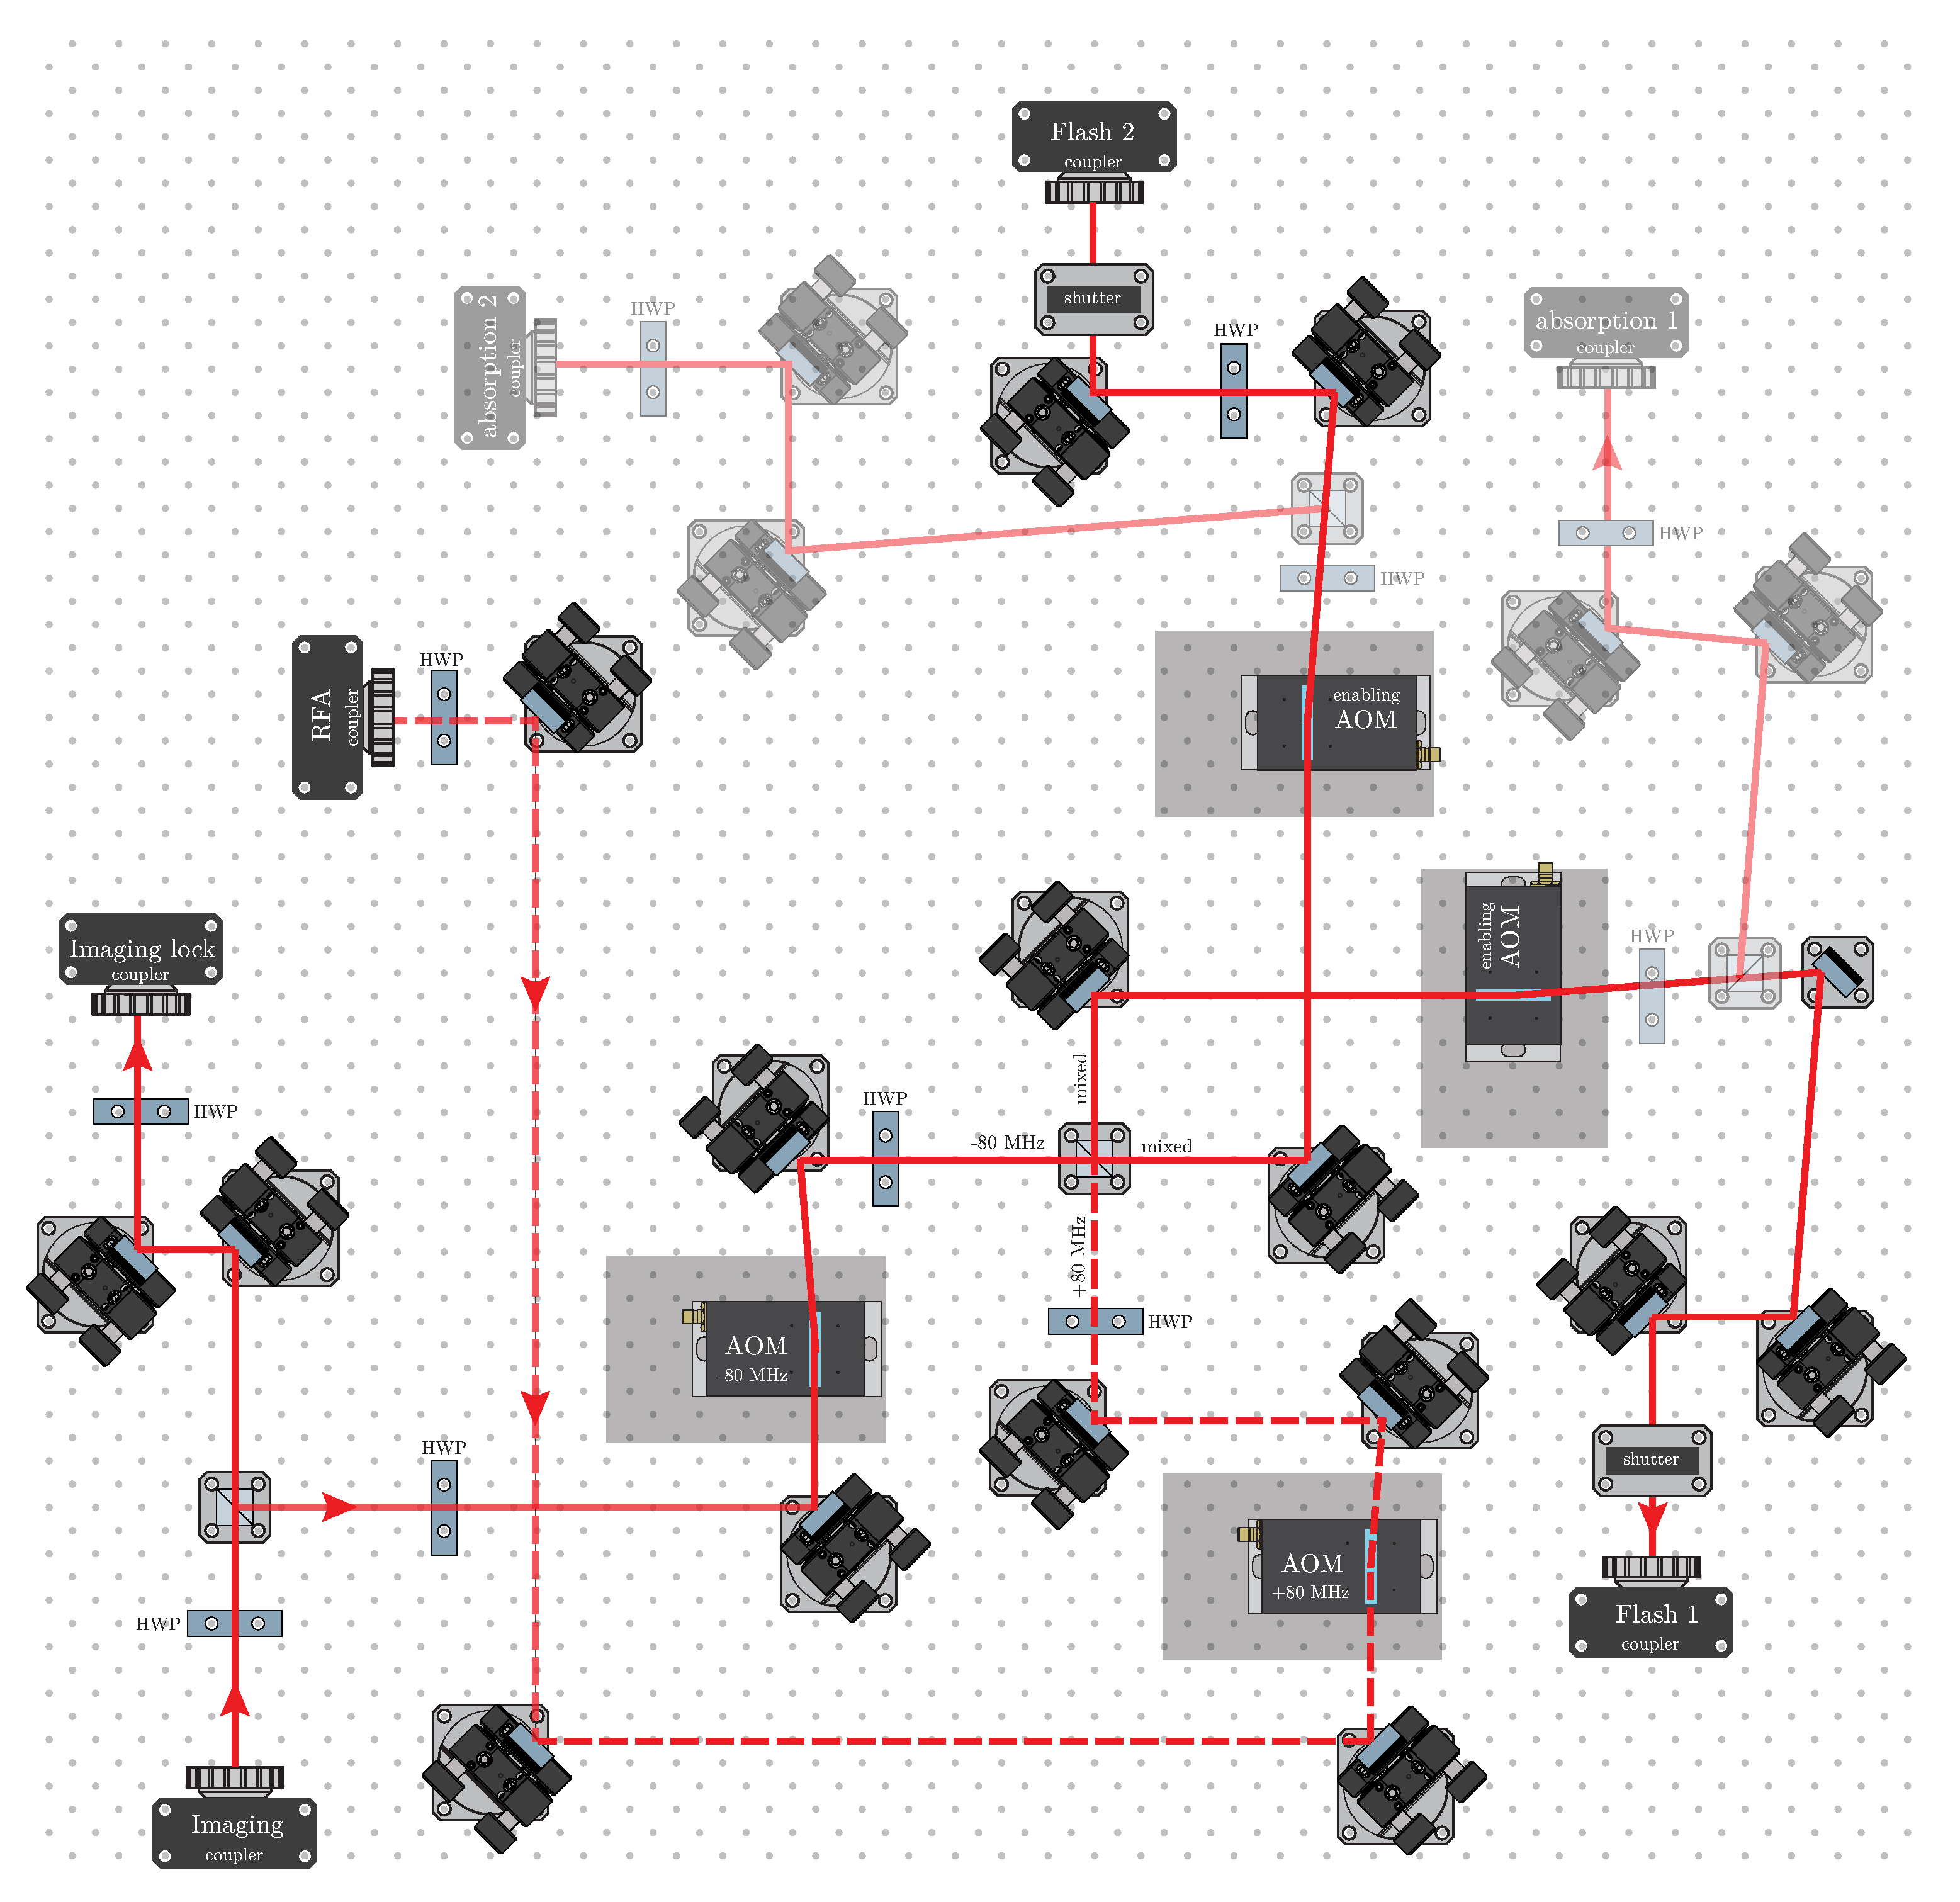
\includegraphics[width=0.4\textwidth]{fig-ai/flashing-distribution-scheme.pdf}
    \hspace{10 mm} 
    \addletter{195}{b} \phantom{4}
    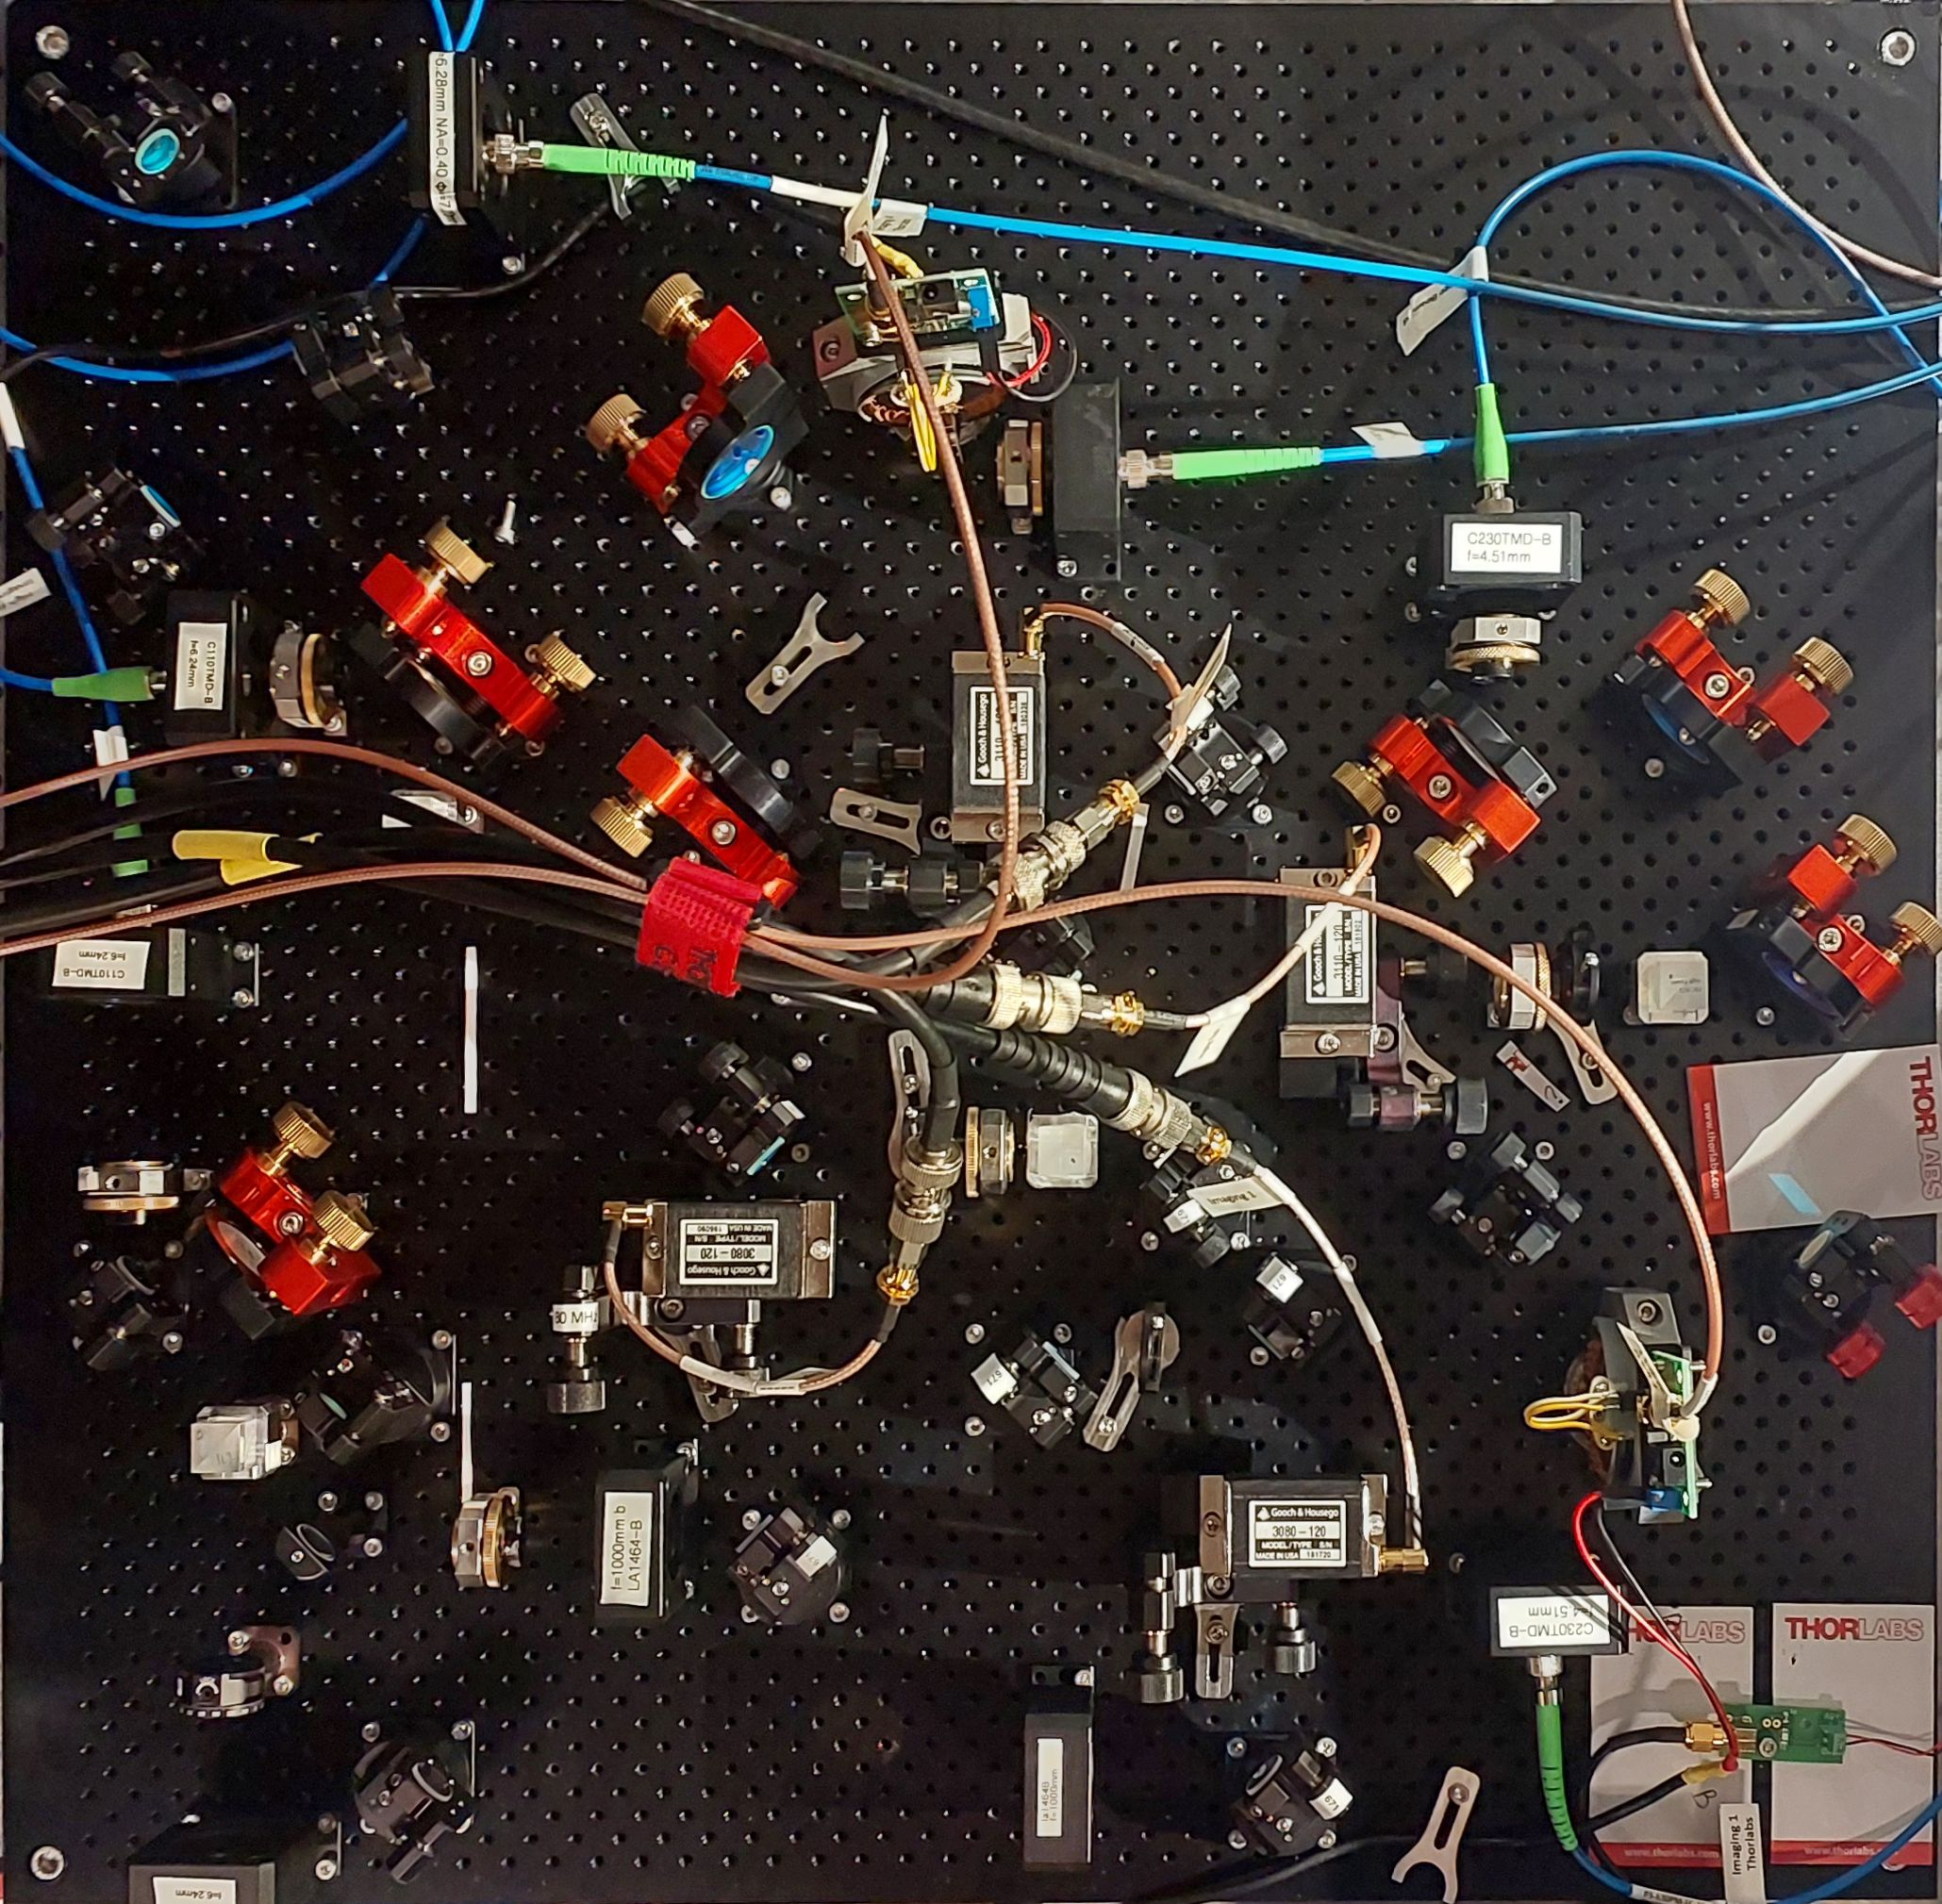
\includegraphics[width=0.4\textwidth]{imgs/flashing-distribution-img.jpg}

    \addletter{90}{c}
    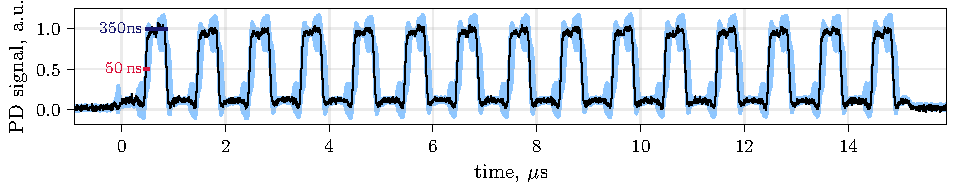
\includegraphics{fig-py/flashing-oscilloscope.pdf}

    \caption{
        \textbf{Distribution board for flashing}. 
        a) Optical layout of the board used to combine and control light for free-space imaging states $\ket{3}$ and $\ket{6}$.
        b) Experimental implementation.
        c) PD signal of the flashing measured on an oscilloscope (black -- a single experimental run, blue -- the standard deviation over 20 runs, red -- rise time).
    }
    \label{fig:flashing}
\end{figure}

% \textbf{Beam combination and modulation.}  
The two lasers are routed through separate enabling AOMs (Gooch \& Housego 3080-120, 120 MHz), which act as fast shutters. The output beams are then combined on a non-polarizing beam splitter (nPBS), producing two spatially overlapping but frequency-distinct outputs. This combination stage is duplicated to form two independent paths, which are later used to illuminate the atoms from opposite directions. Each combined beam is sent through a dedicated flashing AOM (Gooch \& Housego 3080-120, 80 MHz), which controls the on-off modulation during imaging. The modulated light is then coupled into optical fibers, which deliver the light to the main experiment.

% \textbf{Flashing control and synchronization.}  
To suppress recoil-induced diffusion (see Sec.~\ref{subsec:imaging-motivation}), the two beams are pulsed in an alternating sequence. This is achieved by driving the flashing AOMs with square-wave TTL signals at $1~\mathrm{MHz}$, generated by a Rigol waveform generator. The generator itself is triggered by the experimental sequencer (ADwin), ensuring precise timing with respect to the overall shot cycle. Since the imaging beams operate well into the saturation regime, no active power stabilization is required during the imaging sequence.

% \textbf{Beam delivery and geometry.}  
Both beams are collimated and directed onto the atom plane from opposite sides. No focusing optics are used; the beams are weakly converging and approximately collimated over the imaging region. Polarizations are adjusted to match the required $\sigma^+$ or $\sigma^-$ conditions for selective excitation of $\ket{3}$ and $\ket{6}$. Fluorescence is collected through a high-numerical-aperture objective and split by a polarizing beam splitter (PBS), such that the $\sigma^+$ and $\sigma^-$ channels are imaged onto separate regions of the camera. This layout enables single-shot spin resolution (see Fig.~\ref{fig:spin-resolved} and Sec.~\ref{subsec:imaging-spin}).

% \textbf{Implementation and contribution.}  
The distribution board for imaging and RFA beams (including combining optics, AOM stages, and fiber coupling) was fully designed and assembled in the course of this work. This included optical alignment of the two combined beam paths and flashing channels. The downstream delivery system, from fiber coupler to atom plane, was implemented in collaboration with other team members. The beam alignment to atoms was carried out by the author, ensuring symmetric illumination and proper polarization for spin-selective excitation.
